
\section{Data structures and algorithms}
	
%	In this chapter you must describe the data structures and algorithms used in your program. Dont't put your code here, but describe the data structures and algorithms using natural language (you can also add pictures).

	\begin{figure}
		\centering
		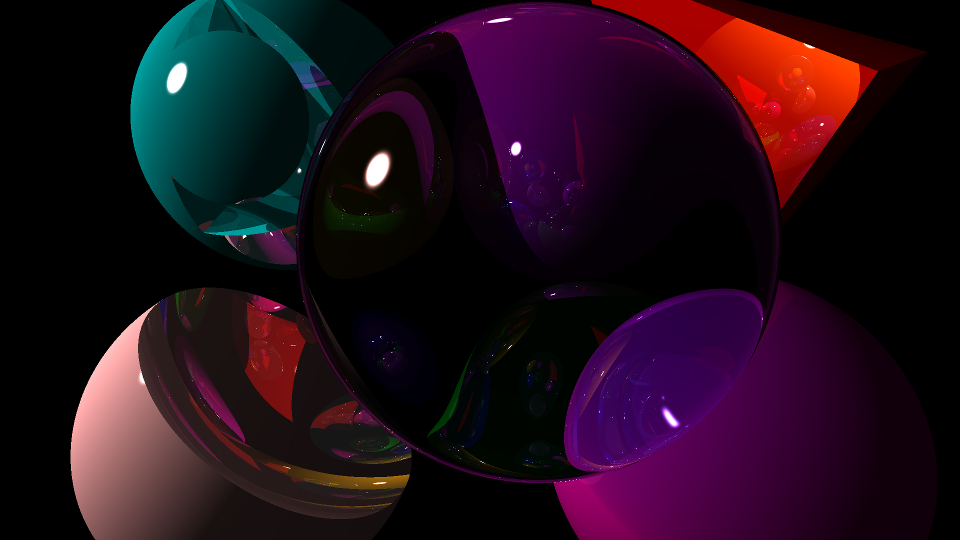
\includegraphics[width=\textwidth]{../img/shapes.png}
		\caption{Example picture}
		\label{f:shape}
	\end{figure}
	
	\subsection{Reading the Scene File}
		
		To build a world using the \emph{FileReading::read(std::istream file)} function a file (or other kind of stream) is needed. The reader reads the stream word by word and uses its \emph{sub}-functions to interpret the objects. All functions make use of the braces, \texttt{\{ \}}. The \texttt{constructive\_solid\_geometry} function uses the same function as the environment \texttt{thing} to add objects to itself. This recursion makes it possible to build complex \emph{CSG}s with many objects.

		The file reader is not necessary to build a World, it can be done through Worlds own functions (also used by the reader), but the scene file input is quite easy and has also helped us a lot with testing.
	
	\subsection{Building the World}
	
		The world is initialized at start-up. Then the different objects (the \emph{Thing}s and \emph{Light}s) in the world are built and added to the world after they are ready. The \emph{camera} is not part of the world, it just makes use of the worlds ray tracing capabilities. That means that many cameras can work on the same World object, and there is only one World per instance of the programme since the class is a singleton.

		The class World as it is built is not capable of moving its objects, just removing and adding new once. 
	
	\subsection{Prepering the Raster}
	
		The whole act of ray-tracing begins from the \emph{Picture} class. Picture had a \emph{Camera} that contains information about the set-up (position, direction, projection, angles, size etc.). The raster (the \emph{Ray}s) for the image is calculated by Picture and sent to the World instance using its function \emph{sendRay}. sendRay returns the colour generated by the ray. All the colours from the rays are stored in a class called \emph{PictureData}.
	
	\subsection{Ray Tracing} 
	
		The class Worlds function sendRay takes a Ray (contains two vectors, origin and direction). sendRay first loops through all the Things in the world and checks, with the Things checkRay function, whether the ray hits it or not. checkRay returns a lu (the length unit used throughout the project) which represents the distance the ray has to travel before hitting the object. From the point where the ray hits the object closest to its starting point (smallest value of the returned lu), if it hits any, three different rays are sent out. The shadow-ray, the reflection-ray and the refraction-ray. All these rays will return a colour and the final colour for send Ray to return is
		\begin{equation}
			c = i_{sh} c_{sh} + i_{rl} c_{rl} + i_{rr}c_{rr}
		\end{equation}
		where the $c$s are the colours and the $i$s the indices of the different phenomena. The $i$s should add up to one. The colour of three different rays are calculated somewhat differently:

		\subsubsection{Shadow-Ray}
			
			The shadow-ray represents the scattered lights. It is calculated for each light source in the world and all the colours added together. The colour contribution from each light source is calculated the following way:
			
			First a base colour is calculated by
			\begin{equation}
				c_{sh,b} = k\frac{c_{mat}c_{light}}{r^2}
			\end{equation}
			where $r$ is the distance to the light and $k$ is a coefficient that we have chosen to be 0.1. After that a ray from the the point to the light is checked for shading objects. If there are any not transparent objects in the way the or if the object itself is in the way of the light only the base colour is returned. If there aren't any objects in the way though a light colour is added to the base colour. The light colour is 
			\begin{equation}\label{e:cshl}
				c_{sh,l} = (1-k)\frac{c_{mat}c_{light}}{r^2}\mathbf{n}\cdot\mathbf{v}_l
			\end{equation}
			where $\mathbf{n}$ is the objects normal in the point and $\mathbf{v}_l$ is the unit vector pointing at the light source from the point.

			If the point is shaded by transparent objects the light in (\ref{e:cshl}) is shaded accordingly.
			
		\subsubsection{Reflection-Ray}
		
			The reflection-rays colour is generated by using the Worlds sendRay function from the point in the opposite direction of the incoming rays mirror image through the objects normal in the point.
		
		\subsubsection{Refraction-Ray}
		
			The refraction-ray goes into the object. The direction is calculated with the formula \cite{maol_sv}
			\begin{equation}\label{e:brytning}
				\frac{\sin \alpha_1}{\sin \alpha_2} = \frac{n_2}{n_1}.
			\end{equation}
			A ray is then sent in that direction through the object and from there it continues in again another direction determined with the same formula (\ref{e:brytning}). The part of the ray that goes through the object is shaded according to the objects materials properties:
			\begin{equation}
				c_{shade} = \left(c_{mat}k_{tansl}\right)^r c_{out ray}
			\end{equation}
			where $k_{transl}$ is the translucence coefficient and $r$ the distance the ray travels in the object. $c_{out ray}$ is the colour of the ray going out on the other side of the object. That colour is again calculated with Worlds sendRay.
		
	
	\subsection{Writing the Image to a File}
	
		At the end the PictureData can write out the colour raster to a simple \texttt{.ppm}-file.
	
	\subsection{Constructive Solid Geometry}
		
		The constructive solid geometry (or CSG) class combines two \emph{SimpleThing}s in one of three different combination types, union, intersection and complement union. A CSG has only one material. The materials in its SimpleThins are ignored. 

		The functions that the CSG needs to be able to calculate for these three types are
		\begin{description}
			\item[checkRay(ray:Ray\&,max:lu):lu] checks if a ray hits the object and returns the distance the ray has to travel before hitting it (returns a negative number if it doesn't hit it).
			\item[checkInnerRay(ray:Ray\&):lu] checks where a ray hits the back wall (ignoring the first surface) the same way as checkRay.
			\item[getNormal(position:Vect\&):Vect] returns a unit vector pointing out of the object. Always called for a point on the surface of the object.
			\item[wraps(position:Vect\&):bool] returns \emph{true} if the position is inside the object.
			\item[onSurfice(position:Vect\&):bool] returns \emph{true} if the position is on the surface of the object.
		\end{description}
		wraps and  onSurfice arn't ever true for the same position. For this a small $\Delta$ constant is used since doubles aren't very exact.
		
		\subsubsection{Union}
		
			In union combination the order of the tow objects doesn't matter. The functions listed above work as follows for unions.

			\begin{description}
				\item[checkRay] calls checkRay for both and returns the smaller positive one (returns a negative number if both ar enegative).
				\item[checkInnerRay] chacks checkInnerRay for both. Returns the positive one if only one is positive (a negative number if both are positive). If both are positive it checks if the smaller ones point is inside the other object (wraps), and if so returns the grater one, else the smaller.
				\item[getNormal] checks on which objects surface the position is (onSurface) an returns the normal (getNormal) from that object and point.
				\item[wraps] returns \emph{true} if wraps is true for either object.
				\item[onSurfice] returns \emph{true} if true fore one of the objects and not inside (wraps) the other object.
			\end{description}
		
		\subsubsection{Intersection}
		
			Intersection is the space occupied by both objects.

			\begin{description}
				\item[checkRay] if positive for both it returns the smaller one.
				\item[checkInnerRay] if positive for both it returns the greater on (with some tweaks for non convex objects).
				\item[getNormal] checks on which objects surface the position is (onSurface) an returns the normal (getNormal) from that object and point.
				\item[wraps] returns \emph{true} if true for both objects.
				\item[onSurfice] returns \emph{true} if true fore one of the objects and inside (wraps) the other object.
			\end{description}
		
		\subsubsection{Complement Union}
		
			Intersection is the space occupied by the first (left) object, but not the second (right).

			\begin{description}
				\item[checkRay] if positive for left it checks if that point is inside right. If so it returns rights checkInnerRay else lefts checkRay. If negative for left if returns a negative number. Except when the ray starts inside left, then rights inner ray is tested and if that point is inside left as well it returns rights inner ray.
				\item[checkInnerRay] if positive for left it checks if that point is inside right. If so it returns rights checkRay else lefts chaeckInnerRay. If negative for left if returns a negative number. Except when the ray starts inside left, then lefts inner ray is tested and if that point is not inside right it returns lefts inner ray.
				\item[getNormal] checks on which objects surface the position is (onSurface) an returns the normal from left if it is left and -normal from right else.
				\item[wraps] returns \emph{true} if true left and false for right.
				\item[onSurfice] returns \emph{true} if true fore left and not inside right or true for right and inside left.
			\end{description}